% 抛物线与弦示意；本图取 p=1、m=0.1，仅示关系，不按比例。
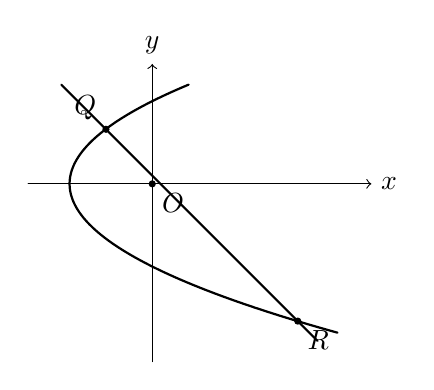
\begin{tikzpicture}[x=1.05cm,y=1.05cm,line cap=round,line join=round]
  \draw[->] (-1.5,0)--(2.65,0) node[right] {$x$};
  \draw[->] (0,-2.15)--(0,1.45) node[above] {$y$};
  \draw[thick,domain=-1.8:1.2,samples=90] plot ({\x*\x-1},{\x});
  \draw[thick,domain=-1.9:1.2,samples=80] plot ({0.1-\x},{\x});
  \fill (0,0) circle (1.3pt) node[below right] {$O$};
  \fill (-0.56,0.66) circle (1.3pt) node[above left] {$Q$};
  \fill (1.76,-1.66) circle (1.3pt) node[below right] {$R$};
\end{tikzpicture}
